\documentclass[12pt,a4paper]{article}
%\usepackage[none]{hyphenat}
\usepackage{graphicx}
\usepackage[margin=2.5cm]{geometry}
\usepackage{listings}
\usepackage{cmap}
\usepackage{afterpage}
%\usepackage{bashful}
%\bash
%texcount -sum -1 tmp.tex
%\END
\usepackage{array}
%\usepackage{nomencl}
\usepackage{float}

\lstdefinestyle{customc}{
  language=JAVA,
  basicstyle=\small\ttfamily,
  numbers=left, 
  breaklines=true
}

\lstset{style=customc}

\begin{document}
\renewcommand{\baselinestretch}{1.50}\normalsize


\title{ An Automatized Analysis to Quantify Collagen Fiber Alignment for Identification of Cancer Biomarkers }
\author{by Alberto Mota Romero \\DENM006: Biomedical Engineering Project \\Supervisor: Dr. Lei Su}

\date{Word count:11,839 \\26 August 2016}
\maketitle
\thispagestyle{empty}

\newpage\null\thispagestyle{empty}\newpage

\newpage
\begin{center}
SCHOOL OF ENGINEERING AND MATERIAL SCIENCE \\[0.3in]

MSc BIOMEDICAL ENGINEERING \\
RESEARCH PROJECT \\
DENM006\\[0.3in]
AUGUST 2016\\[0.3in]
DECLARATION\\[0.5in]
\end{center}

This report entitled:\\[0.1in]

\textbf{An Automatized Analysis to Quantify Collagen Fiber Alignment for Identification of Cancer Biomarkers [0.1in]}

Was composed by me and is based on my own work. Where the work of the others has been used, it is fully acknowledged in the text and in captions to table illustrations. This report has not been submitted for any other qualification.\\

Name: \textbf{Alberto Mota Romero} \\

Signed: \_\_\_\_\_\_\_\_\_\_\_\_\_\_\_\_\_\_\_\_\_\_\_\_ \\

Date: \textbf{26 August 2016}

\thispagestyle{empty}
\newpage

\newpage\null\thispagestyle{empty}\newpage

\LARGE\textbf{Abstract}\\[0.1in]
\normalsize

Fibers arrangements analysis lead to relevant diagnostics, such as the cancer stage. Nowadays, there is not a golden standard to assess the fibers images. Analyse the fibers organizations quantitatively and objectively is fundamental to obtain reliable results. The fibers' features examined were: diameter, length, and orientation angle. Four techniques to assess fibers were implemented and tested. As a result, weaknesses and strengths of each technique were identified. 

\paragraph{}
The CT-FIRE software, developed by the University of Wisconsin-Madison, was adopted as reference. A Single Fiber Isolation (SFI) algorithm was developed to identify individual fiber; as a result, each fiber could be examined separately.  A computer-aided approach measures the fibers characteristic manually in ImageJ. The 2D-FFT spectrum analysis, introduced by Ayres and Levitt, was implemented in an ImageJ plugin. The plugin is available to the public under an open-source license. As the final aim is to classify fibers organizations; additionally, a machine learning classification algorithm was implemented.
 
\paragraph{}
The peak-density parameter is proposed to assess the maximum peak present in the OFD. The peak-density determines the level of fibers organization quantitatively. Fibers organization is a biomarker to identify the cancer stage. The fibers assessed were obtained from two sources: collagen on ovarian cancer tumours and rat-tendon collagen fibers.
\thispagestyle{empty}
\newpage

\newpage\null\thispagestyle{empty}\newpage

\thispagestyle{empty}
\tableofcontents
\thispagestyle{empty}
\thispagestyle{empty}
\newpage
\listoffigures

\listoftables
\thispagestyle{empty}
\newpage

\section*{Notation }


\begin{table}[H]
\begin{center}


\begin{tabular}{ l l }

 \textbf{ OFD } &  Orientation Function  \\
 \textbf{ SFI  } &Single Fiber Isolation  \\
 \textbf{ CT }    & Curvelet Transform  \\
 \textbf{ FIRE  } & Fiber Extraction  \\
 \textbf{ ECM  }  & Extra cellular Matrix  \\
 \textbf{ WHM   } & Width at Half Maximum  \\
 \textbf{ DTAF    } & Dichlorotriazinyl aminofluorescein  \\
 \textbf{ 2D-FFT     } & 2D Fast Fourier’s Transformation  \\
 \textbf{ TACS     } &  Tumour-Associated Collagen Signature  \\
 \textbf{ SHG     } &  Second Harmonic Generation  \\
 \textbf{ NWHM     } &  Normalized Width at Half Maximum  \\
 \textbf{ NABP     } &   Normalized Area Below the Peak \\
 \textbf{ ABP     } &    Area Below the Peak \\
 \textbf{ TABP     } &   Total Area Below the Peak \\
 \textbf{ FW     } &   Full Width \\
 \textbf{ SVM     } &  Support Vector Machine \\
 
\end{tabular}
\end{center}
\end{table}

\thispagestyle{empty}
\newpage





\pagenumbering{arabic}
\section{Introduction}

\subsection{Motivation}

Often, the textile and biomedical sciences have to assess fibers' morphology.  Fibers' length and orientation determine mechanic properties of textile products (Pourdeyhimi, 2002). In the biomedical field, the morphology of fibers is significant for various topics . For instance, the fiber organization determines the interaction between cells and extracellular matrix (ECM) (Ayres, 2008). Thus, for a tissue engineering scaffold, the fibers' morphology determines the cells proliferation and ECM synthesis. Furthermore, collagen fiber orientation is a prognosis of cancer tumor formation (Conklin et al, 2011). In addition, collagen fiber arrangement analysis lead to prognosis tissues disorders, such as osteoarthritis and fibrosis (Chen et. al, 2012). The collagen fiber organization present in the sclerae is matter of study in the glaucoma development (Pijanka ,2012).Identify fiber organization in cutaneous scar tissue is fundamental to understand the cutaneous wound repair(Quinn,2015).

Conklin et al transmit the responsibility of judge the fibers' morphology to humans. Chen et al assessed the images under a computer aided non-automatized technique. The  main challenge is to characterize the fibers arrangement applying an objective, automatized and quantitative method.
\subsection{Objectives}
The first aim is to determine the advantages of each of the different approaches used to analyse fibers organizations. Another objective is to propose and test a new machine learning approach. In addition, an aim is to provide to researchers a tool to assess fibers’ morphology under a quantitative, replicable, objective and automatized procedure.

In addition, this report aims to validate the idea of summarizing the level of fiber alignments under the peak-density parameter. As a result, the fiber alignment could be qualified by a single numeric value.
\subsection{State of art}
The 2D Fast Fourier Transformation (2D-FFT) analysis is a common technique to assess the level of alignment of fibers. Further analysis is required to obtain the quantitative values about the fibers orientation. Ayre anf Levitt suggested a radial summation of the 2D frequency spectrum to obtain the orientation function distribution (OFD). The OFD associates an angle orientation to the quantity of frequency spectrum calculated at that angle. As a result, instead of examining the orientation of fibers from an image, or 2D-FFT spectrum, the OFD graph is analysed. The 2D-FFT procedure has weaknesses; for example, it is concerned by the diameter of the fibers. In addition, the high-frequency components provide non-relevant information; therefore, in order to extract the relevant information, a low-pass filter should be implemented. Tune the low-pass filter could be challenging. Remove components involve losing information about the fibers. The 2D-FFT contributes knowledge about the overall alignment of fibers.

The Hough transform is another mathematical model; it determines the probability of finding a line on an image. The probability is provided for each pair $(r,\theta)$, which defines a line by the equation $r=xcos(\theta)+ysin(\theta)$ .  Although the Hough’s transform is limited to straight lines while the fibers are curved, Pourdeyhimi used this approach. As the 2D-FFT, the Hough transform generates an OFD. However, the Hough transform is computationally more expensive than the 2D-FFT without providing any extra advantage.Pehlke implemented a semi-automatized algorithm to measure the fibers organization with the Fast Discrete Curvelet Transform(2011).

The University of Wisconsin Laboratory for Optical and Computational Instrumentation (LOCI) has produced a complete solution to analyse the fibers morphology. They developed CT-FIRE, an automatized software tool. CT-FIRE is the combination of two algorithms: Curvelet transform (CT) and FIbeR Extraction (FIRE). The FIRE algorithm employs the image intensity to identify each individual fibers. After detecting each fiber, the CT algorithm extracts information about each, such as: length, width, and straightness. The main CT algorithm feature is that it studies the fibers as curves, instead of straight lines; therefore, the results should be more accurate.

\subsubsection{Strengths and weaknesses}

Approaches that involve human intervention to judge the morphology are not optimal for scientific purposes. On the other hand, automatized approaches such as CT-FIRE software and 2D-FFT methods, accomplish the requirements for an automatized, replicable, quantitative and objective assessment of fibers.

The frequency-based approach code, used by Ayres and Levitt, is not available for researchers.  In their papers is provided the methodology, but in order to use it, the user needs to generate the code to implement the algorithm. Furthermore, the approach only provides information about the orientation alignment of the fibers. If researchers require assessing fibers' length and width, another technique must be employed.

CT-FIRE is a fully proved solution; however, it also has a limitation. The FIRE algorithm is not able to distinguish single fibers when they are too thin and dense; therefore, CT-FIRE is not able to provide any result. The CT-FIRE code is available online for free. However, it requires a non-free MATLAB license. Furthermore, many parameters are required to the user in order to run the algorithm. In order to choose variables, users must have a deep understanding of the algorithm, which is a usability limitation. 

Overall, all the approaches require a pre-processing stage to increase the signal-to-noise ration (SNR). The pre-processing stage is fundamental to obtain reliable results. In addition, a further step, proposed in this report,  extract more information from the  OFD functions.

The golden standard solution must be automated, reliable, quantitative and objective. It should be open source, and work for any kind of fiber.  The results must provide information about all morphology parameter, such as: orientation, length, straightness and width. In addition, it must provide summarized parameters to quantify the fibers images. For example, in this report is proposed the peak density as a single parameter to measure the level of fibers alignment.
\subsection{Proposed Approach}
ImageJ is a software widely used to analyse images. The solution presented is an open-source plugin for ImageJ.  The plugin implements the solution based in 2D-FFT, as proposed by Levitt and Ayres.  The output produced is the OFD generation. In addition, the plugin introduces a novel post-analysis process of the OFD graph. The post-analysis stage evaluates the OFD peaks in order to summarize the fibers orientation under a single numeric value.
\section{Theory}
\subsection{Cancer-Collagen Correlation}
Stromal cells and collagen organization are signs of metastasis and tumour formation (Conklin,2011). As a response to the tumour formation, the stromal reacts by increasing the presence of collagen and stromal cells. As a result, the tumour is developed even further.  The stages of breast cancer tumour formation are well described by Conklin et al. First, the membrane surrounding the epithelium breakdown. Then, the stromal collagen matrix is rearranged. Finally, stromal and tumour cells are recruited. In all the stages, the collagen organization has a fundamental function. The collagen organization at each stage is well characterized by tumour-associated collagen signatures (TACS) (Proveranzo, 2006,2008).Actually Grossman et al were able to change the collagen orientation to inhibit the cancer tumor formation(2016).

In the first tumour formation stage, characterized by TACS-1, the amount of collagen increases near to the place where the tumour will grow. After that, on TACS-2, the collagen fibers becomes straight and aligned parallel to the tumour boundary.  At the final stage, the collagen fibers rearrange perpendicular to the tumour , getting a TACS-3. The presence of TACS-3 is relevant because allows an effortless tumour cell invasion into the stroma.Conklin et al found that the aligned collagen is fundamental to facilitate the cancer cells invasion. 

The TACS examination is important to understand the cancer progress. Furthermore, Connklin at al correlated the presence of TACS-3 with the survival rate. The presence of TACS-3 is a biomarker that indicates lower   survival rate. Therefore, a correct interpretation of  collagen fiber images could lead to significant information to diagnosis cancer patients life expectancy.

Besides, the presence of dense collagen is a predisposition state for  cancer development. Thereby, in breast cancer, a dense mastography is an indication of cancer risk. Both, collagen and  stromal generate contrast in X-ray images; so, it is not possible to distinguish the influences of each component. The second harmonic generation (SHG) microscopy generate images based only in the collagen presence. Thus, SHG is a used approach to study the collagen organization during cancer development.



\subsection{Second Harmonic Generation(SHG)}
SHG microscopy is fundamental for the collagen analysis because discloses exclusively the collagen fibers. The SHG has specificity for the collagen without staining or labelling. Only the collagen creates image contrast due to the interaction between the two photons generated with the non-centrosymmetric collagen structure. A narrow bandpass filter centered on one-half the laser wavelength filters the backscattered signal. In order to assess the TACS, the SHG is ideal because the image contrast is generated entirely by collagen. 

The SHG images intensity depends on the fiber thickness and alignment of overlapping fibers (Conkin,2011). Thus, the fibers intensity per se is a parameter to measure the level of fibers alignment. If the fibers are aligned and overlapped, the SHG signal is stronger. Thus, as TACS are based on the alignment of fibers, the SHG images intensity is a useful parameter for evaluating TACS. Walsh assessed the collagen organization using the SHG microscopy due to the SHG predisposition to detect collagen (2015).

\subsection{2D Fourier Transformation as fiber orientation measurement}
The 2D Fourier's transformation is a generalization of 1D Fourier's transformation. The Fourier transformation is because every periodic function is expressed as a series of sines and cosines. Then, the periodic function is represented by the sines-cosines coefficients and frequencies. If a function is non-periodic, it is considered periodic with an infinite period.

The 2D Fourier's transformation is the representation of the 2D signal as a series of 2D sines/cosines function. For simplicity, the sines and cosines could be summarized by the Euler’s notation as:
\begin{equation}
e^{j2\pi(ux+vy))}=cos(2\pi(ux+vy))+jsin(2\pi(ux+vy))
\end{equation}

The Fourier’s transform converts the signals form spatial variables (x,y), to the spatial frequency components (u,v),
\begin{equation}
f(x,y)\leftrightarrow F(u,v)
\end{equation}
Thus, the 2D signal is represented as the summation of sine and cosine with magnitudes denoted by the spatial frequency components F(u,v),  
\begin{equation}
f(x,y)=\int_{-\infty}^{\infty}\int_{-\infty}^{\infty}F(u,v)e^{j2\pi(ux+vy)}
\end{equation}
thereby, the 2D-FFT image represents the frequency  coefficients at the determined pair (u,v). 

Therefore, the image is the sum of complex sine functions as shown in Eq 1. The best strategy to understand the 2D complex sine functions is with examples. The spatial frequencies (u,v), could be represented as a vector. The magnitude of the vector (u,v) determines the spatial frequency at which the represented signal oscillates. On the other hand, the vector's direction is parallel to the direction at which the periodic signal is moving. In the vector's direction, the signal changes; while in the perpendicular direction the signal remains constant. 

In fig. 1 is plotted the magnitudes of an example of a complex signal defined by eq. 1 at arbitraries values of frequency pairs u and v. The function represents parallel periodic gradients. The combinations of the frequency components (u,v), analysed as vectors, determines the direction, and spatial frequency of the lines gradients. The lines gradient alignment is perpendicular to the direction of the vector defined by the frequency components (u,v). As the magnitude of the vector increases, the lines are repeated at a faster spatial frequency. 

The signal's 2D-FFT shown in fig. 1 should be two points that represent the pair of (u,v) at which the complex signal was calculated. However, due to the limitations of the representation (discrete space and quantification intensity values), the empirical transformation is not two perfect dots, but two points are distinguishable (fig. 2). In the fig. 2, the separation of the dots, related to the magnitude of the generated vector (u,v), is proportional to the spatial frequency of the counterpart in fig. 1.1.  The direction of an imaginary vector drawn from the origin (center) to the points is perpendicular to the direction of the lines shown on figure 1. 

The idea of the Fourier's transform is that the superposition of the complex functions (eq. 2) can reconstruct the original image. The magnitude of the Fourier transformation |F(u,v)| , represents  the amplitude required for each complex signal (eq. 1), at the specific pair (u,v). Therefore, the high amplitude of a frequency pair component indicates high intensities of the pixels oriented at that direction. This feature is the key to assess the fibers orientation using the Fourier’s transformation. 

If an image's 2D-FFT has high components for a specific pair (u,v),  it indicates that the signal generated by the frequency components (u,v)  is fundamental for the formation of the image. So, the image should have many high-intensity pixels in the perpendicular direction of the vector generated by the point (u,v) with respect the origin. Thereby, the fibers on the image must be aligned perpendicular to the vector (u,v).

If the vector's (u,v) magnitude is high is because the complex signal represent thin lines. The high magnitude components could represent thin fibers or noise. A threshold must be selected to decide below which vector's (u,v) magnitude the components could be considered part of the fibers.

\begin{figure}
  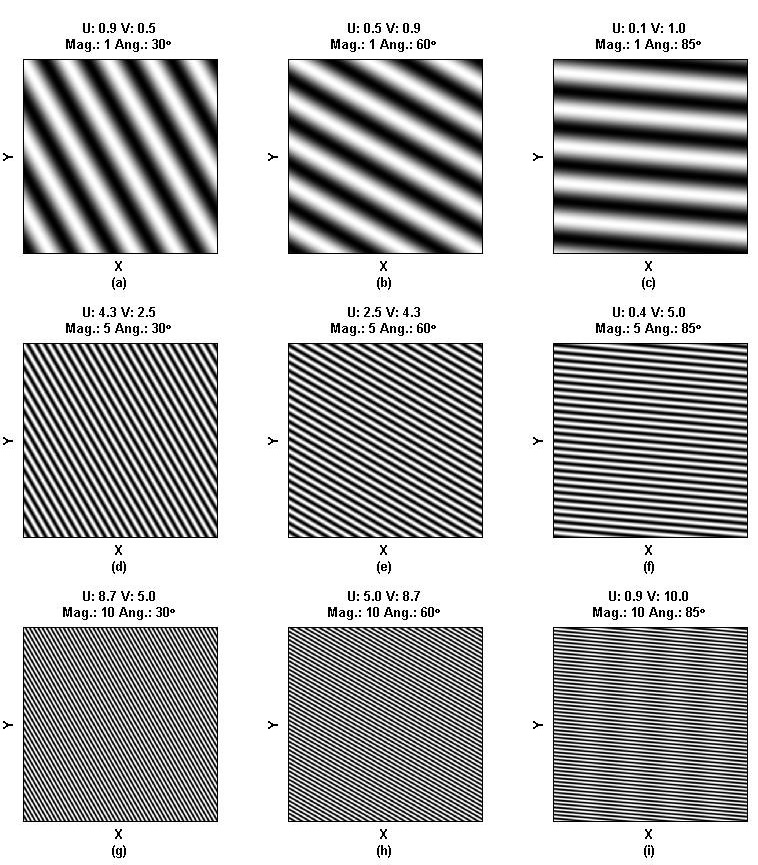
\includegraphics[width=\linewidth]{FiguresDisertation/figure1.jpg}
  \caption{2D Complex Signals}
  \medskip
  \small
  Plots a, b and c have a vector (u,v) with magnitude 1; thus the width of the lines are constant. The angles direction vectors have values of 30⁰,60⁰, and 85⁰, respectively; therefore, the orientation of the lines variates perpendicular to the angles directions. Images (d,e,f) are generated by a vector (u,v)  with a higher magnitude,(magnitude=5); as a result, the gradient's frequency increase. The samples obtained from vectors with magnitude 10, has the highest spatial frequency (g,h,i).
\end{figure}

\begin{figure}
  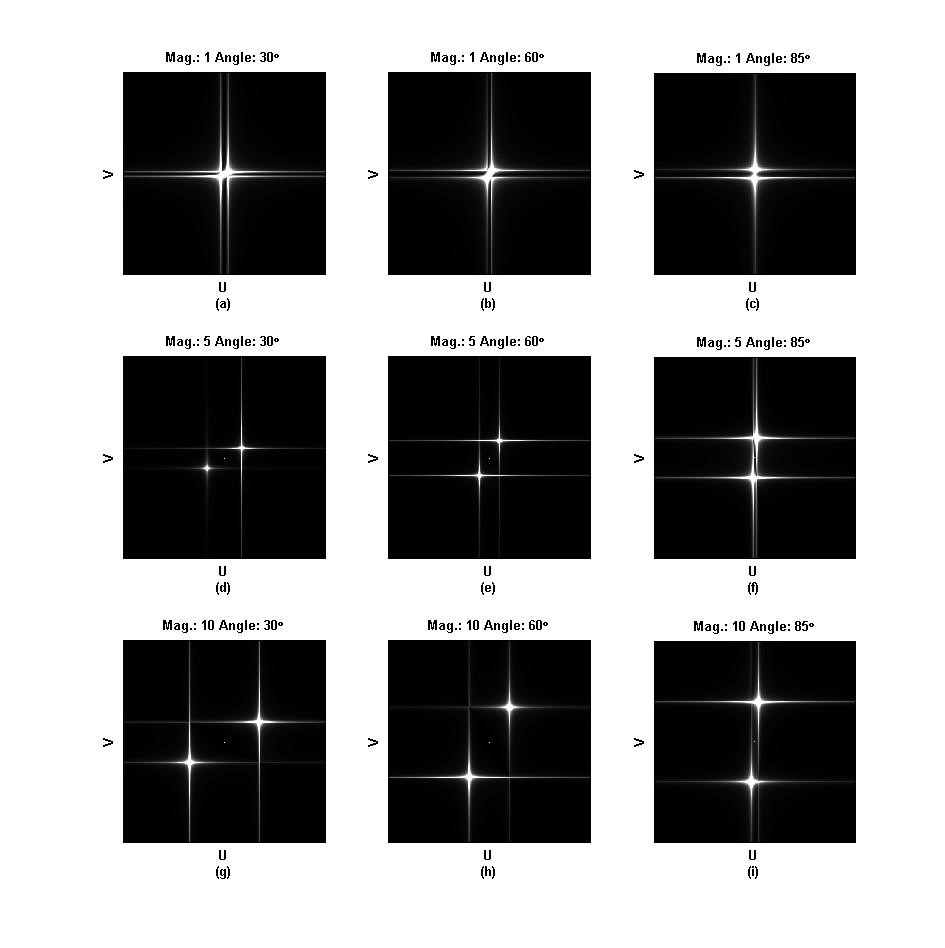
\includegraphics[width=\linewidth]{FiguresDisertation/figure2.jpg}
  \caption{Fourier's spectum of one-component 2D complex signals}
  \medskip
  \small
  Fourier’s transforms counterpart of the functions shown in fig. 1.  As the magnitude increase, the separation between the dots increases. The direction of a vector drawn from the origin (center) to the dots is perpendicular to the lines generated in the counterpart plots in fig 1. The closest the dots, the shortest the magnitude, so the line's spatial frequency is slower.
  %\label{fig:boat1}
\end{figure}
\subsection{Fiber Extraction}
Develop an automatized computational fiber isolation algorithm is a heavy challenge. FIRE algorithm (Stein,2008) is based on previous studies of Wu et al (2003) to detect 3D fibers networks. For 2D Images, a simplified approach is used to assess fiber networks. In summary, the theory consists in detect network nodes based on the distance from the pixels to the background. A long separation between pixels to the backgrounds indicates the pixel is a network node. Then, the network nodes are connected to identify fibers. 

Once the network nodes are associated, is straightforward to obtain the fibers straightness, angle orientation, length, and width. Lastly,  statistical information is obtained about the general fiber morphology. However, the statistical weight of each fiber is equal independently of the area each  fiber occupies on the image. 

\subsection{Pre-processing Image}
A pre-processing step to prepare the image for the actual analysis improves the final results (Ayres, 2008). The image preparation removes noise; so, the SNR increases. Thus, it is helpful for all approaches: fiber extraction and Fourier’s spectrum analysis.  For all images, the pre-processing removes noise by eroding and dilating the images. Furthermore, for 2d-FFT analysis, it also serves as a low-pass filter.  The erode-dilation process removes the high-frequency components, which are representative of too thin lines components. On the other hand, the fibers erosion-dilatation process should be tuned to avoid mistaking noisy groups of pixels as fibers.

The erosion process of an image A by a matrix B, needs B moving within the image A. Every time that the matrix B fully matches the values inside the image A, the pixels are retained; otherwise, the pixels are deleted. Thus, the small noisy groups of pixels that are not large enough to fulfil the matrix B are deleted. If a group of pixels cannot fulfil the matrix B, it must not be a fiber.  Pixels at the edge do not match fully the matrix B; therefore, the edges of the fibers are undesirably deleted. In order to restore edge pixels, the dilation morphology algorithm restores them.  

The dilation process is the antithesis of the erosion. The matrix B moves inside the image A; if an image pixel matches the matrix B at the center, the pixels are retained or added to the image will. Thus, the removed pixels of the edges of the fibers are restored in the image.

The low-pass band filter is implemented by defining a cut-off frequency. All the components with a higher than the frequency are removed. As a result, only low-frequency components, which are characteristic of fibers, remain for the proper analysis.  Complementarily, as a finer filter, a dilate-erosion algorithm removes isolated groups of high-frequency components below the cut-off frequency.

\subsection{Machine Learning Classification}
Supervised machine learning classifiers are adaptive algorithms to generate predictions based on datasets provided. The classifier algorithms prognosticate the group at which future dataset belongs.  The workflow first consists in extract datasets from test-images. The test-image's classification is well known. The datasets of each image are obtained from the images' features. The technique utilized to get images' features is called 'bag of words'. Then, the model is trained, to archive a model able to predict. The training was performed by different techniques such as: 'Linear Discriminant Analysis','Fine Gaussian Support Vector Machine', and 'Simple Decision Tree'. 

\subsubsection{Bag Of Words}
Visual-word is a concept to characterize images.All images contain characteristic matrixes of pixels. Each matrix of pixels is a visual-word. A bag-of-words is a set of unique visual-words. The set of visual-words is extracted from several images. Then, each image is characterized by an array specifying the number of repetition of each visual-word inside an image. Bag-of-words technique is employed in machine learning algorithm to characterize images. 

\subsubsection{Support Vector Machine}

The Support Vector Machine (SVM) is a machine learning technique for classification. The idea is to find the most suitable hyperplane possible to separate the classes. The hyperplane must isolate all the data points for one group.It is an hyperplane because each data point depends on many variables; for example, an array generated by the bag-of-words.

\subsubsection{Simple Decision Tree}
A decision tree is a structure of conditions to archive a resolution. The tree has internal nodes with conditions/tests to select a route along the tree's branches.  As the algorithm reach the end of a branch a decision is archived, In this case, the decision trees are based on the dataset provided for each image. The decision desired is the group to which each image belongs.  

\subsubsection{Linear Discriminant Analysis}

The Linear Discriminant approach is based on the analysis of variance, regression analysis, principal component analysis and factor analysis. It search for a linear combination of values to characterize each aggrupation. The weighted sum of the characteristics parameters generates a unique value, discriminant, to describe the image. So the images could be classified based on the discriminant.

\section{Methods}
\subsection{Images sources}
Images were supplied by: Dr. Delaine-Smith and Dr. Rowson. The  Dr. Delaine-Smith's images were obtained using a Second Harmonic Generation (SHG) microscopy from metastatic ovarian tumours biopsies. The samples were fixed and  embedded in paraffin. Finally, they were ordered into tumour microarray.  Dr. Rowson's images were obtained from rat-tail tendon fascicles stained with DTAF. DTAF stains proteins, which are primarily presents in collagen.

\subsection{Pre-Processing Stage}
\subsubsection{Binarization}
The threshold used to perform the binarization was calculated by the Otsu’s method. In order to obtain the orientation, length, straightness and diameter, the image intensities are not relevant. Actually, the binarization of the image provides a 2D-FFT cleaner of high-frequency components because the grey-scales components are deleted.
\subsubsection{Erosion and dilation}
The pre-processing's main objective is to remove noise from the image. The binarization removes the pixels that do not have enough intensity to be considered as fiber-pixels. The main source of noise after the binarization is the presence of collagen dots. Therefore, as explained in the previous section, the erosion process removes the small dots of collagen, which are not part of any fiber.

The matrix to perform the erosion and dilation were performed by a matrix of 5 by 5 pixels. Some images have more noise pixels than others do; thus, the number of erosion-dilation repetitions should be customized to each image. The plugin developed for ImageJ, allows the user to decide the quantity of erosion or dilation process that must be performed to remove the noise. The automatized version performs the erosion-dilation process three times.
\subsection{Fibers Orientation}

In the ImageJ plugin, the fiber orientation assessment is obtained through a Fourier’s transformation approach. First, Fourier's transformation is approximated by the images' 2D-FFT. The FFT is an algorithm to reduce the computational cost of obtaining the Fourier’s transformation. The 2D-FFT algorithm requires an extra step to rearrange the zero-frequency component to the center of the image.

As demonstrated in the previous section the Fourier's transformation generate a frequency spectrum that is perpendicular to the overall fiber orientation. Accordingly, to keep it straightforward, the 2D-FFT spectrums were rotated 90 degrees. Consequently, the fibers and the Fourier’s spectrum are oriented in a parallel direction.

The next step, was to determine in which direction is oriented the Fourier’s spectrum. Following the Ayres and Levitt approach, the radial summation of the frequency spectrum at every Δθ degrees was calculated. As a result, every $\Delta\theta$ degrees, from $0^{\circ}$ to $180^{\circ}$ the radial summation of the Fourier’s spectrum determines the level of orientation at that specific angle. The level of orientation as a function of the degrees is called OFD.  The OFDs shown on this report were computed at a $\Delta\theta = 0.5^{\circ}$. The ImgaeJ allows the user to select the preferred $\Delta\theta$.

\begin{figure}
  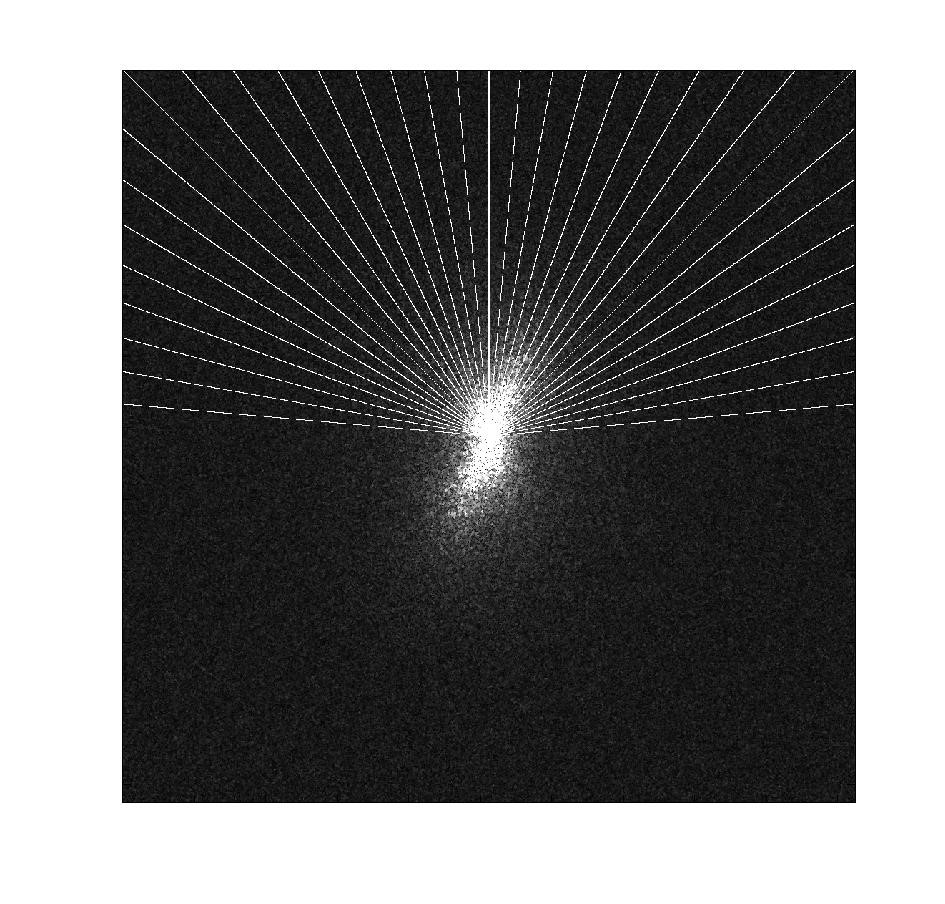
\includegraphics[width=\linewidth]{FiguresDisertation/figure3.jpg}
  \caption{Radial frequency spectrum sumation}
 \medskip
  \small
  The pixels are summed radially to obtain the respective value of the OFD at each angle. In the image is shown an example of angles taken every $5^{\circ}$. In practice, the OFD was calculated every $0.5^{\circ}$.
\end{figure}

As the OFD can be plotted; it provides an easier data presentation. A graph is easier to assess than an image.  An OFD plot provides a clearer data presentation, so is easier determine the fibers orientation angle. On the other hand, OFDs could have random peaks, which could mislead conclusions. Peaks analysis produces more reliable and quantitative information about the fibers orientation. From the  OFD peak analysis could be obtained the peak density parameter, which provides information about the level of fiber arrangement.

\subsubsection{Peak Density}

The aim of assessing the OFD peaks is to determine whether a peak contains a representative amount of the OFD´s signal power. The OFD peak density validates if the area below the peak is substantial in comparison to the total area below the OFD.  The peak-density  could be defined as the Normalized Area Below the Peak (NABP) over the Normalized Width at Half Maximum (NWHM):
\begin{equation}
PD=\frac{NABP}{NWHM}
\end{equation}
The width at half maximum (WHM) is defined by the distance between the peak's nearest right and left points that are half the maximum peak's normalized amplitude. The normalized amplitude of the maximum peak is the magnitude of the maximum normalized with respect the minimum value.  Accordingly, the NWHM is the WHM normalized with respect the Full Width (FW):
\begin{equation}
NWHM=\frac{WHM}{FW}
\end{equation}
The ABP is the Area Below the Peak within the WHM. The ABP is normalized with respect the Total Area Below the Curve (TABC) defined by the OFD,
\begin{equation}
NABP=\frac{ABP}{TABC}
\end{equation}
The purpose of the normalization is to obtain unitless parameters. As a result, the comparison of parameters between different OFDs is independent of the OFDs intensity values.

\subsubsection{Example: SHG Metastatic Ovarian Tumours}
Nine images provided by Dr. Delaine-Smith’s were assessed. The images are presentative of nine cases of fiber organizations. Six images show fibers clearly oriented fibers, while three of them has fibers with no orientation. A human can distinguish oriented from non-oriented fibers. 

\begin{figure}
  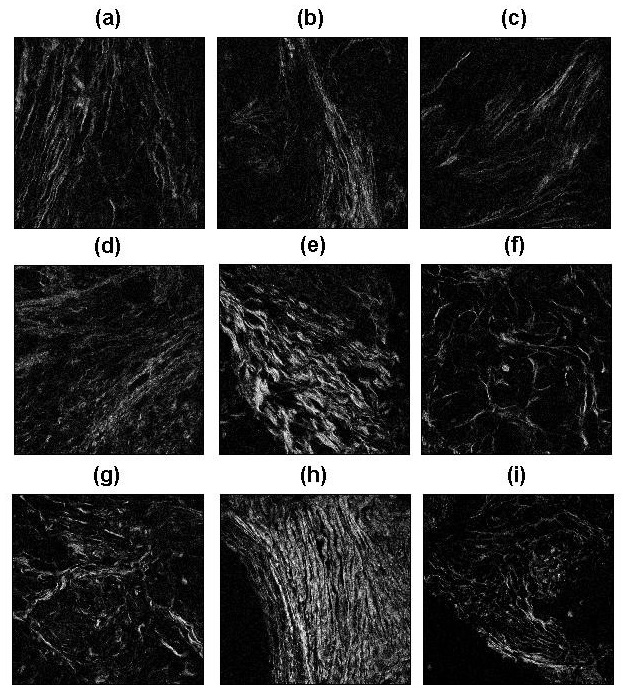
\includegraphics[width=\linewidth]{FiguresDisertation/figure4.jpg}
  \caption{Collagen in Ovarian Cancer Tumours }
  \medskip
  \small
  Fibers in images a, b and h are oriented in a vertical direction, while c, d, and e in a diagonal direction. On the other hand, images f, g and i are randomly oriented. The purpose of the algorithm is to determine the fibers orientation angle quantitatively. Besides, the OFD peak density parameter indicates whether the orientation level of the fibers. Images provided by Dr. Delaine-Smith.
\end{figure}

The images' frequency spectrums of the oriented fibers have an elliptic morphology oriented perpendicular to the general orientation of the fibers. On the other hand, the non-oriented fiber images have a circular frequency spectrum. The Fourier's transformation contains high-frequency components that can be removed, as those are not representative of the fibers.

\begin{figure}
  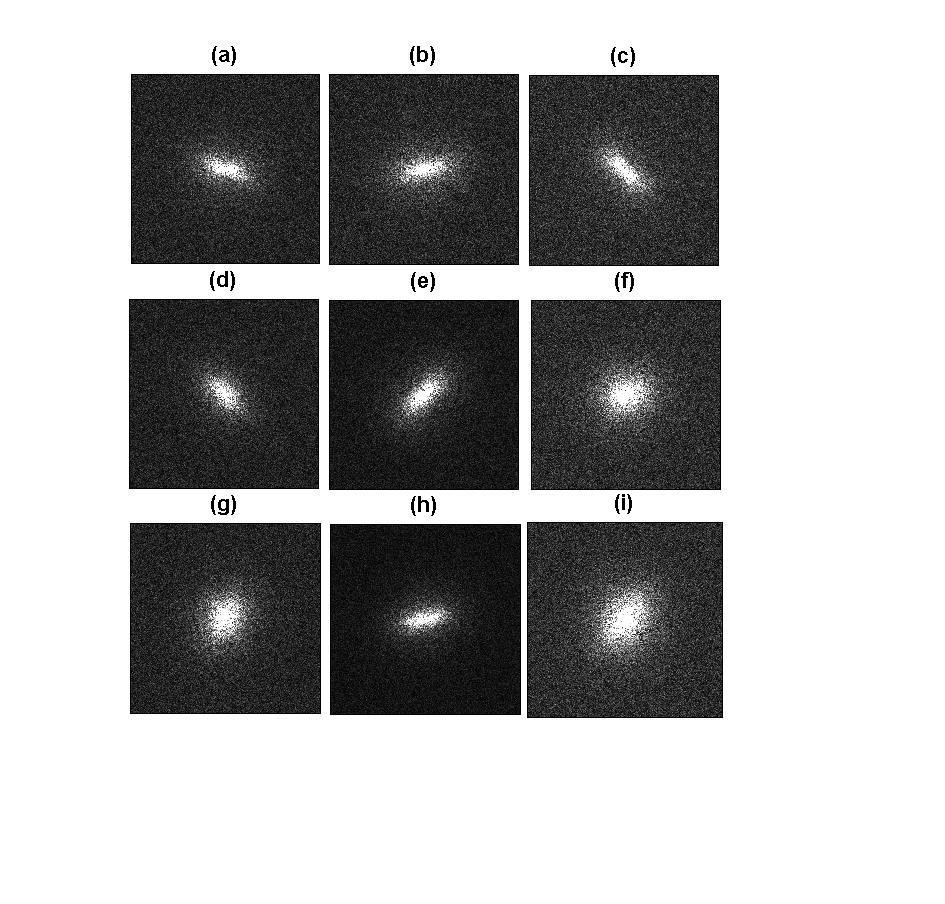
\includegraphics[width=\linewidth]{FiguresDisertation/figure5.jpg}
  \caption{Ovarian Cancer Tumours 2D-FFT. }
  \medskip
  \small
  Corresponding Fourier's representation of the images shown in figure 4. The fibers vertically oriented have a horizontal spectrum (a,b,h). The fibers diagonally oriented (c,d,e) have frequency-spectrum oriented perpendicularly. The randomly oriented fibers' spectrums (g, f, i) resembles circles, instead of oriented ellipses.
  
\end{figure}

First, a low-pass filter removed the highest frequency components. Then, high-frequency components were removed repeating erosion-dilation processes with a 10-by-10 square stencil. The erosion-dilation method removes small groups of high-frequency components. Due to the erosion algorithm nature, if there is an outstanding group of high frequencies, the values are retained.

The Fourier's spectrum is rotated $90^{\circ}$, so it becomes parallel to the  fibers arrangement. After that, the OFD was calculated by making radial summations of the frequency spectrum. The OFD is smoothed with a rolling average of five elements. Once the OFD is computed, the peaks assessment is performed to determine the level of fiber orientation at the maximum orientation angle.

\begin{figure}
  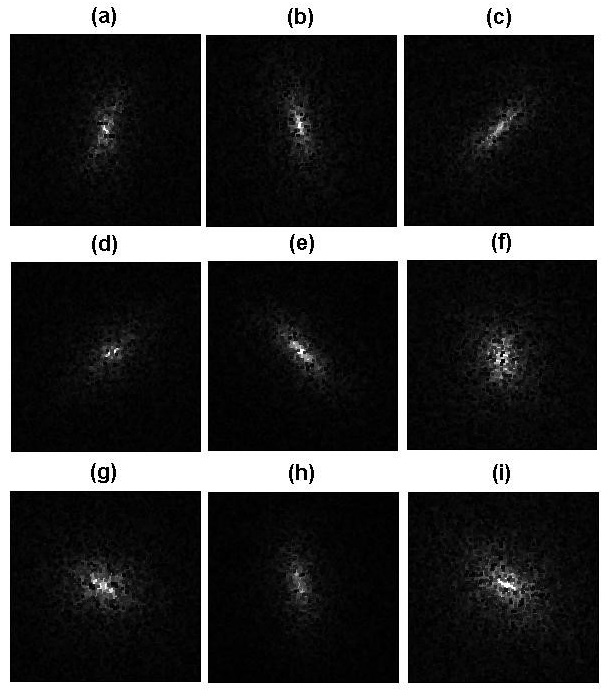
\includegraphics[width=\linewidth]{FiguresDisertation/figure6.jpg}
  \caption{Ovarian Cancer Tumours 2D-FFT after low-pass band filtration.}
  \medskip
  \small
  The Fourier's spectrums are filtrated because the high-frequency components are not essential for the reconstruction of the fiber's image . The frequency spectrum is rotated $90^{\circ}$ to make the 2D-FFT spectrum orientation parallel to the actual fibers orientation.
\end{figure}
\subsection{Fiber's Length and Diameter}
In order to examine the fibers length, diameter, and straightness, the fibers must be analysed individually. After the pre-processing stage, the pseudo-fibers are removed; then, the actual fibers could be isolated. The own implemented algorithm to identify individual fibers is based on groups of contiguous pixels. If pixels are adjacent, they are assumed to be part of the same fiber. However, in to be more accurate, when two fibers overlap, the network analysis proposed by Stein et al is required.

Once the fibers are identified individually, each fiber is surrounded by the tiniest ellipse possible. The smallest ellipse's minimum and maximum axis are associated with the fiber's length and width. The approximation of fibers as ellipses generate errors. 

\subsection{Single Fiber Isolation}

In comparison to the FIRE’s algorithm, a simpler fiber detection algorithm was implemented. Pixels that are adjacent and in on-state are grouped as a single fiber. In contemplation to evaluate the fiber’s length and width the smallest ellips, surrounding the group of pixels is found. The major axis of the ellipses approximates the length, while the minor axis proximate the width. Besides, the fibers orientation is achieved from the ellipse's orientation. The orientation angle is obtained with respect the ellipse’s major axis.
\subsection{Human-Computer Aid Analysis}

Chen et al. assessed the fibers' orientations using ImageJ. The user traced a line in the same direction than a fiber; then, ImageJ measures the line angle of the drawn line. However, the fibers are oriented in many directions. The user must draw lines in the same direction that most of the fibers. In spite of evaluating the human-computer aid approach, for each image, twenty lines were drawn parallel to the fibers. The lines' angle mean was assumed the main orientation angle. The main orientation angle is the parameter to compare with the other approaches.

The principal disadvantage of the human-computer aid analysis is that it relies on the human judgment. It depends on the limited amount of samples evaluated. The person has to choose which fibers to appraise. Furthermore, the fibers are considered as straight lines, but actually, they are curves.

\subsection{Machine Learning Classification}

In order to identify TACS-3 fiber organization, is necessary to decide if the fibers are aligned. A machine learning classification to determine whether the fibers are aligned or not was run implemented under the MATLAB  Statistics and Machine Learning Toolbox.

The machine learning success depends on the correct model and a number of samples. The number of images is limited. The rat tendons images were not enough to perform the test on them. The ovarian cancer tumour set of images contains 27 images. Machine learning approach requires two set of models: one to train the model, and the other to test the model. Even 27 images are few images. The training set of images had 18 images and the last 9 images were used to test.

A bag-of-word of 200 elements were obtained from the train-set to characterize each image. As a result, each image was represented by a characteristic-array. Each characteristic-array contains 200 numbers registering the repetitions of each word inside the image. Additionally, the OFD and peak density were attached to the characteristic-array.

The training set of images were classified as aligned and unaligned by the human judgment. Then, the  models were trained by using tree techniques:'Linear Discriminant Analysis','Fine Gaussian Support Vector Machine', and 'Simple Decision Tree'. The models were trained automatically by the MATLAB Statistics and Machine Learning Toolbox.  The influence of human judgment is never desired. 

For the same images, two datasets were trained seeded by different features. One dataset was feed with the 200 visual-words; while the second dataset was feed with the peak-density and OFDs values (mean, standard deviation, maximum and minimum).

\subsection{Software Development}
First, the algorithms were implemented in MATLAB for quickly debugging, as a proof of concept. However, as MATLAB is not an open source platform, then, the algorithms were implemented using Python. The Python implementation presents some disadvantages for the users, because it requires the Python and dependencies installation to run. Therefore, in order to provide a more user-friendly solution, a plugin for ImageJ was developed. The ImageJ plugin was developed in Java. ImageJ is a popular software in the scientist community to analyse images. Moreover, ImageJ has a tested full interface to manage images.

\section{Results}
\subsection{Fiber Orientation}
\subsubsection{SHG Metastic Ovarian Tumours}

Of the fig. 4, images f, g and i are randomly oriented; thus, the corresponding OFD's maximum peak density, are short values in comparison to the measured from well-oriented fibers. Empirically, the images with non-oriented fibers use to have a maximum peak density less than 1.2. 

Images of fig. 4 that could be inferred as 'vertically-oriented' (a,b,h), have peak density values above 1.2, and orientation angles close to $90^{\circ}$. As expected, the values are not exactly  $90^{\circ}$  because the fibers are not precisely oriented at  $90^{\circ}$ . The orientation angle is a precise angle, instead of an ambiguous 'vertically-oriented' judgment.  

The images judged as diagonally oriented (c,d,e), has orientation angle values close to  $45^{\circ}$ or  $135^{\circ}$. Also, they present a maximum peak density greater than 1.2. Moreover, two numeric values were calculated to describe images features that could be used to identify TACS quantitatively.


\begin{figure}
  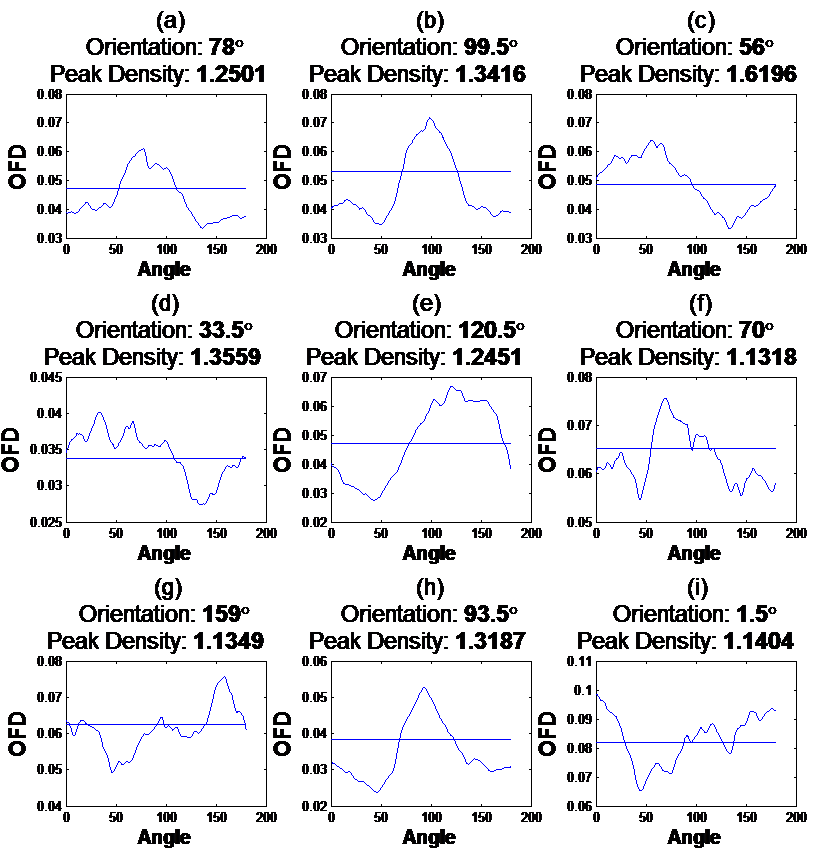
\includegraphics[width=\linewidth]{FiguresDisertation/figure7.png}
  \caption{OFDs Ovarian Cancer Tumours Collagen}
  \medskip
  \small
  The fig. 4 and fig. 5 corresponding OFDs. Non-oriented fibers (f, g and i) have peak density values less than 1.2; so, although they have an orientation angle, the fibers are not truly oriented. The horizontal line shown in each graph represents the middle between the maximum and minimum value, at where is calculate the WHM.
  
\end{figure}

\subsubsection{Rat tail tendon fascicles}
\begin{figure}
  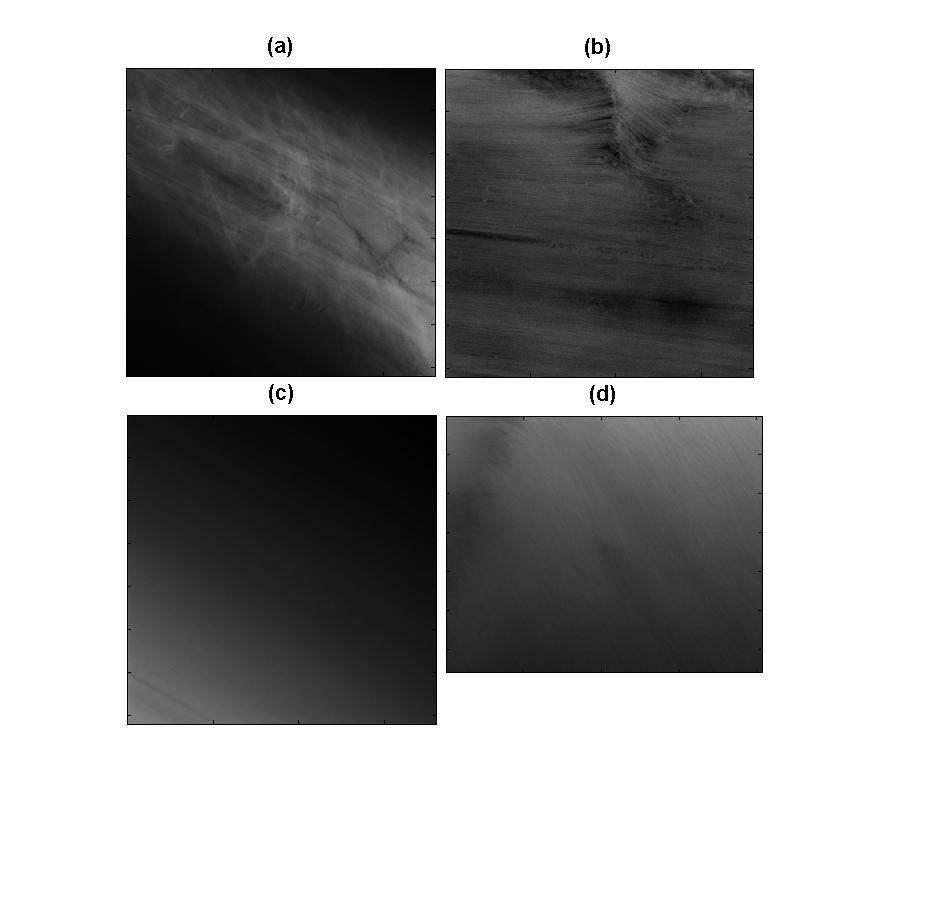
\includegraphics[width=\linewidth]{FiguresDisertation/figure8.jpg}
  \caption{Rat tail tendon fascicles stained with DTAF}
  \medskip
  \small
  Rat-tail tendons have thin collagen fibers at distinct orientations. The fibers are uniformly oriented. The thin fibers are an obstacle for FIRE to distinguish individual fibers. Neither the developed algorithm is capable of isolating the fibers.
  
\end{figure}

In comparison to the ovarian tumours, the tendon fibers are oriented more uniformly; as a result, the peak densities are higher. The orientation angles are congruent with the images. Images (a) and (c) (on fig. 8) are close to $150^{\circ}$, while (b) is almost horizontal with an orientation angle of $178^{\circ}$. Finally, (d) is more vertical than (a) and (b); thus, it orientation angle is $116^{\circ}$.

\begin{figure}
  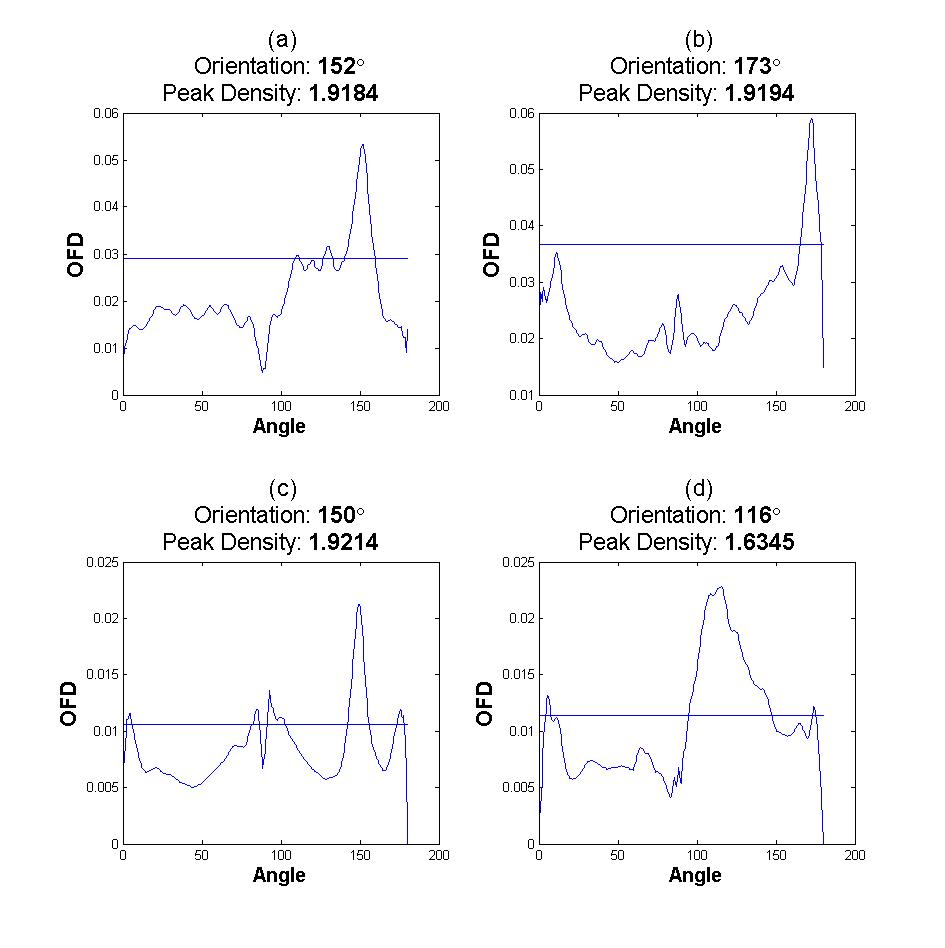
\includegraphics[width=\linewidth]{FiguresDisertation/figure9.png}
  \caption{Rat Tail Tendon Fascicles OFD }
  \medskip
  \small
  The rat-tail tendons fascicles images generate sharper OFD’s peaks than the generated from  ovarian tumours images.
\end{figure}

In contrast with the tumour's OFDs, the OFDs for the tail tendons have better-defined peaks; as a result, the peak density values are greater as well. Furthermore, the highest tumour's peak density value is less than the lowest rat tendon's peak density value.

\subsection{Comparision}
\subsubsection{CT-FIRE(Ovarian Tumours)}

The results are satisfactory for the human judgment: however, it is better to compare results with a reference. As there is not a golden standard to analyse fiber images; so, CT-FIRE results are used as a reference. The CT-FIRE implements a completely different approach than the Fourier analysis. The CT-FIRE distinguish each fiber to analyse it individually. Finally, a statistical analysis generates overall information about the fibers organization. 


\begin{table}[]
\begin{center}
\begin{tabular}{ |c|c| }
\hline
 \textbf{ Fourier's Approach Results} & \textbf{CT-FIRE Results} \\
\hline
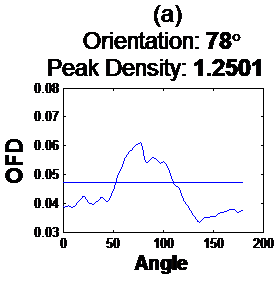
\includegraphics[width=0.5\linewidth, trim=0 0 0 -10]{FiguresDisertation/t1a.png} &
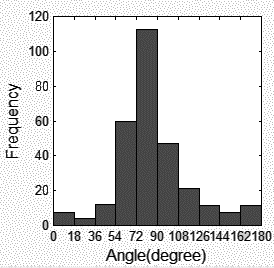
\includegraphics[width=0.5\linewidth, trim=0 0 0 -10]{FiguresDisertation/t1b.png} \\
\hline
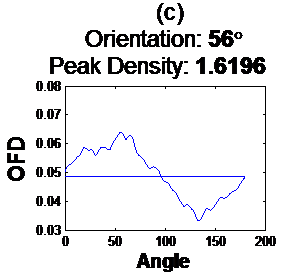
\includegraphics[width=0.5\linewidth, trim=0 0 0 -10]{FiguresDisertation/t1c.png} &
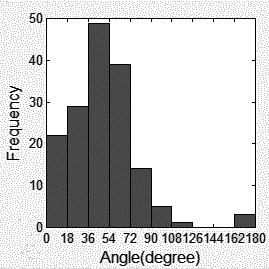
\includegraphics[width=0.5\linewidth, trim=0 0 0 -10]{FiguresDisertation/t1d.png} \\
\hline
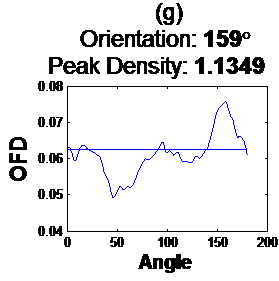
\includegraphics[width=0.5\linewidth, trim=0 0 0 -10]{FiguresDisertation/t1e.png} &
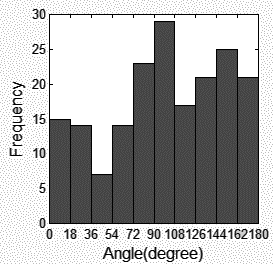
\includegraphics[width=0.5\linewidth, trim=0 0 0 -10]{FiguresDisertation/t1f.png} \\
\hline    
\end{tabular}
\end{center}
\caption{CT-FIRE comparision against 2D-FFT Approach}
\end{table}

The angle at which the Fourier's OFD's has a maximum was compared with the CT-FIRE angle mode. The error of the Fourier's approach with respect CT-FIRE's results is of the 6.9\%.

\subsubsection{Single Fiber Isolation (SFI) Results (Ovarian Tumours)}
The ovarian tumours images are suitable to distinguish individual fibers. The amount of fibers identified with the SFI algorithm is less than the distinguished by CT-FIRE. In the SFI, the fibers are approximated as ellipses. The angle orientation results only differs $\pm5.3^{\circ}$ from the Fourier’s analysis results.

The principal objective of implementing the SFI algorithm was to obtain a technique to have a method to measure the fiber width and length. These values were compared with the CT-FIRE results. Withal, in comparison to CT-FIRE results, Student’s t-test reveal the data were not statistical significant equally, nor different. One-sample T-tests was performed to compare the results with the Fourier’s analysis, with the same inconclusive results.

The SFI orientation angle average error is 8.8\% with respect the CT-FIRE results. The mode of the SFI orientation angle was compared to the CT-FIRE results. The average diameter error with respect CT-FIRE´s results is 55\%.  On the other hand, the length error is 9.6\%. The width error value is due to the different approaches to measure the diameter. The SFI uses a rough approximation (ellipse) to measure the width at the minor axis.

\subsubsection{Human-Computer Aid (Ovarian Tumours) }
Chen et al. conducted a human computational aid approach to examine the fibers. In order to have an extra reference, other than CT-FIRE, a human-computational aid technique was implemented. For each image,  twenty representative fibers were assessed for length, width, and orientation.

The computationally aided approach error for width and length, in reference to CT-FIRE results, is greater than 30\%.  The fiber's width is not uniform along the fibers, so the judge was encouraged to measure the shortest fiber width. Although the width's error is around 30\%, it represents 1-pixel error because the ovarian tumours fibers are in average 4-pixels width. The length error increases because human judges have a bias to measure long fibers, as it is easier.

Regarding the orientation analysis, the computationally aided approach error is 9.8\%, with respect CT-FIRE’s results. Human judges intuitively measure the overall direction of the fibers. CT-FIRE results manage the short and large fibers equally, which could misconduct the general orientation angle results.

\subsubsection{Overall Comparision (Ovarian Tumours)  }

The SFI and CT-FIRE results were compared using Student’s t-test. The t-test indicates the datasets can not be considered statistically different nor equal. A one-sample t-test compared the CT-FIRE orientation datasets against the computer-aid and 2D-FFT results. The results were not conclusive. Therefore, the errors with respect CT-FIRE results were calculated. 

The SFI and computationally aided fiber width results differ from the CT-FIRE’s results in 30\% and 55\% respectively. The human judgment and the number of samples limit the computational-aid analysis. SFI’s results are farther (55\%), because they are calculated under the fiber-ellipse approximation. The ellipse’s minor axis is assumed as the diameter; however, the minor axis is even wider than the thicker cross-section distance along the fiber.

The SFI length results are less than a tolerable 10\% error. Contrarily, the computer-aids length results are 50\% far from the CT-FIRE results. Although the judge should measure long and shorts fibers indistinctly, there is a bias to measure long fibers. Meassure the long fibers is easier. The automatized approaches do not dismiss the short fibers; sometimes, avoid the short fibers could be desired.

All the angle orientation results,  for all analysis approaches, are in an error range below 10\%, in comparison to CT-FIRE. The computer-aid results are farther from the CT-FIRE results because the computer-aid approach does not take into consideration the small fibers. However, for some analysis, the short fibers effect could be undesired. Perhaps, the examination only requires information about the long fibers orientation. The Fourier’s technique results are the closest to the CT-FIRE results.

\begin {table}[H]
\begin{center}
\begin{tabular}{ |c|c|c|c| }
\hline
 & \bf{Fourier's Approach} & \bf{SFI} & \bf{Computer Aid} \\
 \hline
 \bf{Width} & ----- & 55\% & 30\% \\ 
 \hline
 \bf{Length} & ----- & 9.6\% & 50\% \\ 
 \hline
 \bf{Orientation Angle} & 6.9\% & 8.8\% & 9.8\% \\ 
\hline    
\end{tabular}
\caption {Techniques comparisions against CT-FIRE results.}
\footnotesize
\begin{flushleft}
Fibers diameter is the most challenging parameter to measure. The orientation angle was obtained within an error range always below to 10\%. The computational-aid approach provides only reasonable values about the angle orientation (9.8\%). Therefore, to measure the length only CT-FIRE and SFI (9.6\%) lead to consistent results. The Fourier’s approach is not capable of extracting information about the diameter and length.
\end{flushleft}

\end{center} 
\end {table}

\subsection{Rat Tendons Images}

In contrast with the tumours fibers, the rat tendons fibers are too thin. Moreover, the distance between fibers is shorter. Besides, the fibers population density is higher. Even for the human is challenging distinguish individual fibers. So, CT-FIRE and SFI are not capable of identifying individual fibers. Therefore, no results were obtained from the rat tendon images using these techniques.

Only two techniques could analyse the tendon fibers: Fourier's approach and computationally-aid analysis. Thus, only these techniques were compared statistically. Improvements on the fibers identifier algorithm would enable the CT-FIRE or SFI analysis. 

\subsubsection{CT-FIRE Results (Rat Tendons)}

The CT-FIRE algorithm relies on the individual fibers identification, but the rat’s tendon fibers are too thin and dense (fig.8). Consequently, the CT-FIRE was not able to provide any information about the images.

\subsubsection{Fourier’s Approach (Rat Tendons)}

For tendon images, the computer-aid results are the unique comparable reference. Fig. 9  shows the 2D-FFT results. All the tendons OFDs have a peak-density higher than 1.6, a value that ensures the fibers are highly oriented.

\subsubsection{Human-Computer Aid (Rat Tendons)}

In a computer-aid analysis, only a limited number of fibers are assessed. As the fibers are too thin, the diameter could not be measured because the fibers are indistinguishable. Fibers length could not be measured because the fibers start and finish out of the image. The range of vision is too short to estimate the length. 

\subsubsection{Overall comparison (Rat Tendons)}

Tendon fibers were assessed only for angle orientation. Only the Fourier’s and computer-aid results were compared. The error between the two techniques is 4.6\%. Although the error is relatively low, the one-sample t-test cannot conclude a significant equality nor difference.

The orientation angle error (4.6\%) is within a tolerable range. The computer-aid test is tricky because the fibers are not distinguishable by the human eye. However, in order to measure the orientation is not required to distinguish each fiber; the judge can draw lines parallel to the groups of fibers.

\subsection{Machine Learning Classification}

Two datasets were tested: 200 visual-word based and peak-density based. The  statistical and peak-density approach had better results independently of the classification learning technique, table3.


\begin {table}[H]
\begin{center}
\begin{tabular}{ |c|c|c| }
\hline
  \bf{Classifier} & \bf{Visual-word based} & \bf{Peak-density based} \\
 \hline
 \bf{Simple Decision Tree} & 85.7\% & 100\% \\ 
 \hline
 \bf{Linear Discriminant} & 92.9 & 100\%  \\ 
 \hline
 \bf{SVM} & 64.3\% & 92.9\%  \\ 
\hline    
\end{tabular}
\caption {Machine Learning Classifier precision comparison.}
\footnotesize
\begin{flushleft}
Although the visual-word based dataset has 200 values to characterize the images, the peak-density based dataset, with only four values, is more reliable. 
\end{flushleft}

\end{center} 
\end {table}

The peak-density dataset reaches a 100\% of accuracy classifying images; however, this result could mislead due to the few quantity of samples. More samples must be tested to obtain more reliable results. Every machine learning approach improves its accuracy with the peak-density model. 

\subsection{ImageJ plugin}

The ImageJ plugin was developed to facilitate researchers the analysis of fibers. The plugin was designed to be user-friendly. Only two parameters could be customized: degrees separation and binarization threshold. By default, the binarization threshold is calculated dynamically with the Otsu´s method. If it is required, it could be defined by the user, selecting the checkbox “Binary Thres.”. The “degrees of separation” is $\Delta\theta$ ; the separation in degrees between the imaginary lines drawn to calculate the summation of  the frequency spectrum. The shorter $\Delta\theta$, the more accuracy archived.  In consequence, also the computational time required is longer.

The plugin can be executed in two modes: automatic and step-by-step mode. The step-by-step mode allows the user to observe the partial results along the process. The automatic mode, runs the full algorithm at the background; it is easier for the user. The step-by-step mode allows customization of the erode-dilation process; as a result, it can obtain images without noise and Fourier´s transform without irrelevant high-frequency components. 

\begin{figure}
  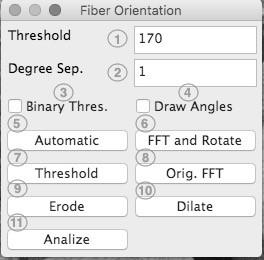
\includegraphics[width=\linewidth]{FiguresDisertation/figure10o9.jpg}
  \caption{ImageJ Plugin User-interface}
  \medskip
  \small
  ImageJ plugin user-interface to perform image analysis based on the Fourier´s approach. (1) Customizable threshold to binarize the image, only when (3) is checked. (4) Show the lines drawn at $\Delta\theta$,  to add up the frequency components (purely informative).(5) Runs the entire algorithm on the background. (7) Binarize the image. (6) The first step in the process: calculates the 2D-FFT and rotates the image $90^{\circ}$. (9,10) Enable the user to perform the erosion and dilate process. (8) Recovers the original 2D-FFT, after any dilation and erosion procedures. (11) Analyse the 2D-FFT after the erode-dilate procedure, by adding the frequency components at the respective angle
\end{figure}

For academic understanding, the plugin has the option to draw the imaginary lines along where the frequency components are added (Fig. 10-4 ). The erosion and dilation procedures could be run as many times as required for each image. If it is necessary to recover the original 2D-FFT, it can be recovered quickly (fig. 10-8). The final step is to add the frequency components in radial directions(fig. 10-11). The results archived are the:  OFD and OFD's peak-density. 


\subsection{Accuracy}

The SHG sensitivity is high enough to measure fibril's diameters (Bancelin et.al, 2014). Therefore, the images are not an accuracy limitation to measuring diameter and length. On the other hand, the technique to measure the diameter could limit the precision of the obtained values. Approximate the diameter as the ellipse's minor axis of is not an accurate approximation. The diameter measured by a person in ImageJ neither, as the diameter should be measured at the narrower section.

The SFI algorithm's accuracy could be improved by using another technique to measure fibers diameter. Also, the algorithm to distinguish individual fiber needs further improvements. Even the CT-FIRE is not able of identifying all fibers. CT-FIRE and SFI use to mistake groups of fibers a single one. 

CT-FIRE has a dedicated algorithm to analyse fibers as curves, CT (curvlet transform). The rest of the approaches assume the fibers are straight lines. Approximate curves as straight lines produce an error. The error is greater when the fibers present more curvature. Even the 2D-FFT analysis measure the pixels orientation in linear straight directions, no curves. 

\section{Discussion}
\subsection{Fibers as curves}

The Fourier’s spectrum represents images as a summation of complex signals. Each frequency component denotes periodic diagonal lines at different angles. The SFI examine each fiber individually as an elliptic approximation. The ellipse's axis estimates the fibers length and diameter. The computer-aid analysis assesses the fibers by drawn lines by humans. All approximations are a source of inaccuracy. Analysing fibers as straight lines is another approximation. CT-Fire is the unique approach presented in this report that study the fibers as curves. 

The root problem becomes from the idea of try to describe a fiber orientation by an angle. A line could be characterized by an angle, but fiber could have different shapes, which could not be represented by an angle. Conveniently, the Fourier’s OFD peak-density is a parameter to measure the level of fibers overall organization, independently of the angle of orientation.  Orientation angle is entirely dependent on the position where the image was taken. The angle must be measured in reference to a specific location; for example, a tumour. Only if the angle is referenced to something, the orientation angle could be a significant parameter. 

Therefore, the OFD peak-density is a primary parameter to assess the level of fiber arrangement. The peak-density could become a parameter to diagnostic TACS.  It is independent of the location at where the photo was obtained. In general, researches that assess the level of fiber organization could be based on the peak-density value. 

\subsection{Orientation Angle Length Weighted}

The images have fibers of many lengths and orientations. Algorithms that extract fibers for individual analysis (CT-FIRE and SFI), does not take into account the length of the fiber when the orientation angle is calculated. For these techniques, all fibers have the same statistical weight to calculate the angle orientation, independently that some fibers occupy more space in the image. If the image has fewer long fibers than tiny fibers, the results would indicate that the main orientation is given by the tiny fibers, no matter that the tiny fibers hold an irrelevant area portion.
  
It would be more representative to weight the orientation of each fiber by its length. Then, the angle of the biggest fibers (which occupy larger area in the image) orientation angle would have a greater impact in the overall angle. On the other hand, the 2D-FFT approach interpret the images as a whole; thus, the longest fibers influence more the frequency spectrum than shorter fibers. 

\subsection{Fiber detection challenge}
The SFI algorithm is too basic to detect fibers overlapping. The CT-FIRE is capable of detecting networks of overlapping fibers by finding “nuclear points”, points where the fibers intersect. The nuclear points are detected thanks to the distance from the pixel to the background. After a second “nuclear point” is spotted, the algorithm moves along the direction diverging from the nuclear point. It is a complex and reliable algorithm; even though, the some of the detected fibers are split. 

The 2D-FFT analysis does not have to detect each fiber for the analysis. Therefore, for images with thin and dense fibers, as the provided by Dr. Rowson, the analysis could be performed. CT-FIRE software is not able to identify that kind of fibers; so, no results are obtained. For images with non-identifiable fibers, the width and length could only be measured by computational-aid systems, for now. 

Meanwhile, to measure fibers width and length is necessary to detect individual fibers. Therefore, the fibers detector algorithm must be improved to be able to extract fibers from any image. Also, the technique to analyse each fiber has to be adjusted to obtain more reliable measurements of width and length. Machine learning could learn about the variety of fibers arrangments; so a general algorithm to detect fibers on images could be archived.

\subsection{Alignment Level}
The angle orientation per se, does not provide relevant information; unless the location where the image was taken is referenced to a certain point. For example, the fibers could be at $60^{\circ}$ in the image, but that could indicate the fibers are perpendicular to a tumor. The fibers angle with respect a point could be an important parameter to understand collagen metabolic behaviors.

Independently of the image’s location and position, the fibers organization level is a relevant parameter for different purposes. The OFD's peak-density quantify the fibers arrangement level to the same direction. For the textile industry, the alignment level could be enough to determine the textiles quality. An advanced cancer stage is correlated to the aligned arrangement of fibers, TACS-3. The OFD’s peak-density is archived using the Fourier’s approach. If the images are not referenced to a particular point, the peak-density still provides relevant information about the fibers morphology. Thus, the peak-density could be a fundamental parameter to validate quantitatively research hypothesis.

\subsection{Diameter Assessment Challenge}
Fiber's diameter is measured at the shortest width of the 2D projected fiber.  For the computer–aid, analysis is complicated to find the shortest diameter; as a result, the error increases. Furthermore, the diameter in the ovarian cancer tumors is in the order of four pixels; so, a single pixel error denotes a 25\% variation. As a result, the fiber’s diameter error becomes a startling high value.  

For SFI results, the diameter error is worse than the length error. The smallest ellipse surrounding the fibers is an approximation of the fiber. The ellipse's major axis approximate the fiber's length and the minor axis the fiber's width. However, the ellipse´s width is changing along the ellipse. The ellipse’s minor axis has to be larger than the thinner section of the ellipse surrounding the fiber's extremes. Thus, the minor-axis is always larger than the real diameter. A mathematical adjustment could improve the accuracy of the approximation. Moreover, the pseudo-fibers detected by the SFI should be analyzed by a network detector algorithm, as CT-FIRE, to obtain the shortest diameter along the fiber.

\subsection{Image  Preprocessing}
\subsubsection{Binarization}
The aim of the binarization process is to distinguish the remove background noise. The simplest technique is choosing a threshold; then, all pixels with an intensity below the threshold are turned off. The idea is that all pixel with a lower intensity than the threshold are considered noise, so they removed. As different images could have a variety of intensities, select the threshold could be a challenge. The Otsus´s method is an adaptable, simple and functional method to choose the threshold. There were not complications due to the binarization process.

\subsubsection{Morphological Dilation-Erosion}
The dilation-erosion process's objective is to remove noise remaining after the binarization process. The erosion algorithm removes small groups of pixels which are not fibers. However, it also shrinks the fibers. The dilation process restores the lost pixels. A balance between erosion and dilation must be archived. Different images require customized amounts of erosion-dilation processes. The developed ImageJ plugin by defaults performs the pair dilation-erosion algorithm three times. 

The high-frequency components do not contain relevant information about the fibers; therefore, they should be removed. A low-pass filter removes the highest frequency components. The selection of the cut-off frequency varies image to image. The high-frequency components are present as isolated groups of pixels; thus, they can be removed with erosion-dilation process. The erosion-dilation process should be tuned for each case. The plugin by defaults performs the pair dilation-erosion algorithm three times. In addition, the user could run the dilation or erosion processes as many times as required.

\subsection{Fourier’s Analysis Approach}
The Fourier's analysis approach is independent to the fibers diameters. It does not depend on the capability to identify individual fibers. Adversely, it does not provide information about the fibers' length and diameter. The fibers arrangement results are less than 10\% different in comparison to the CT-FIRE results. 

Although the Fourier's analysis approach is a reliable and robust, the low-pass band filter must be adaptive to different 2D-FFTs. The default dilation-erosion setup provided acceptable results, but customized filters could lead to cleaner results. The ImageJ plugin is an excellent tool to experiment with the filtering process because it enables the user to run the erosion and dilation process as many times as desired. 

The ImageJ plugin is an implementation of the technique used by Ayres. The novel feature is the post-analysis, the OFD's peak-density to evaluate the level fibers arrangement. The peak's density assesses quantitatively and objectively the OFD. As the peak-density is a parameter that evaluates the level of fiber organization, it could be employed to diagnosis cancer stage or any other metabolic process correlated to fibers organization. Also, in the textile industry could be used to determine textile quality.

The Fourier's transform analyses the overall image. The 2D-FFT components reconstruct the images taking into consideration the fibers curves. So, independently of the curves, the results provide general information about the fibers orientation.

\subsection{CT-FIRE}
CT-FIRE is a reliable solution with few limitations. The principal strengths are the: robust fiber extraction algorithm (FIRE), and the fibers analysis as curves (CT). The curvelet transform (CT) analyses each fiber as curves instead of lines. Subsequently, the results are more precise.

On the other hand, identify fibers for thin and dense arrangements is a challenge. For example, the rat-tendons fibers are thin and dense-populated; thus, the CT-FIRE is not able to extract them. In those cases, the Fourier's approach is an alternative, but only for orientation assessment. Only the human-computer technique could measure fiber's width and length. Further development of fiber identification algorithms could solve this limitation. 

In order to run CT-FIRE  algorithm, around 20 parameters should be provided by the user; therefore, the user should understand how the algorithm works. User's lack of knowledge about the algorithm could become an obstacle. A user's manual is available online(http://loci.wisc.edu/files/loci/software /ctFIRE\%20Beta\%20V1.2.1\%20Users\%20Manual.pdf) 

Analyze the fibers as curves is useful because the length is measured more accurately. In addition, the curvelet analysis enables the fiber straightness evaluation. However,  the CT-FIRE reported angle is the angle of a line traced from the initial to the final fiber's points. The fiber's angle reported is an approximation by the line's angle. 

\subsection{Single Fiber Isolation}

SFI is a process completely automatized. SFI has many areas of opportunity. For example, examine the fibers as curves instead of straight lines. Also, rather than assume that the group of pixels in the neighborhood are a single fiber, networks of fibers should be discovered, as CT-FIRE.

Once a set of pixels is categorized as an individual fiber, the smallest ellipse surrounding the group of pixels is determined. The major axis is an approximation of the fiber´s length. The minor axis is an estimate of the fiber´s length. Approximate a fiber as an ellipse is a rough assumption. The approximation error due the diameter approximation is huge because the minor axis has to be longer than the fiber´s thickest section. As the thickest section is farther from the fiber's center, the error becomes greater.

Furthermore, the ovarian cancer fiber's width is in average 4 pixels long; thus, small differences reproduce high percent error. Correspondingly, the ellipse's major axis is longer has the fiber's lengths as the ellipse surround the fiber completely. 

Future development should improve the fiber detector algorithms. Isolate thin and dense arrangments is a challenge. The pre-processing stage is an area of opportunity to overcome this limitation. The elliptic estimation should be enhanced by a more reliable approximation. Also, the fiber network detection algorithm should be achieved.

\subsection{Computer Aid Analysis}

Chen et al examined the images utilizing ImageJ. The technique consists of drawing lines to measure the fibers parameters (orientation angle, length, and width). The human involvement in the process adds limitations. Humans are not able to assess features at images with thin indistinguishable fibers. In populated organizations, the judge can only assess a limited number of fibers. Analyse several fibers for many images is time-consuming. Thus, only fibers samples are assessed; as a result, an equivalent to “shot noise” is produced. In addition, as the process is not automatized, the reproducibility is limited.

The human judgment has a bias to assess the long fibers because they are more accessible. As a result, the short fibers values, which are the majority, are ignored. In contrast, the automatized approaches examine all the fibers indiscriminately. For computer-aid, analysis, the results about the fibers length are misconducting because only the long fibers are measured. The orientation angle measured is also guided by the long fibers, which could be desired because long fibers occupy a larger area of the image.  Besides, the reproducibility is limited because the process is not automatized.   

The fiber diameter must be measured on the shortest fiber's cross-section. For a human is troublesome find the shortest cross-section width. Some diameters measured with ImageJ are not the wanted. Thus, the results are not reliable. The human intervention in the process restricts the process reproducibility.  

\subsection{Absence of standard}

Summarize the orientation of several fibers in a single value leads to losing information about the image. Also, is misconducting assign a numeric value to describes the length and diameter of many fibers as those values fluctuate for each image. The peak, mean and standard deviation describe further the features.

The 2D projection of a 3D fibers mesh does not show certainly individual fibers. Therefore, for a human is tough to distinguish each fiber.  Even for the software algorithm identify individual fibers is a challenge. Hence, there is not a standard to measure fiber's parameters.

In the absence of a golden standard, there is not comparison reference. However, CT-FIRE was used as a reference. CT-FIRE results are fiable because it has been tested and used in previous researches. CT-FIRE is developed by the Laboratory of Optics and Computational Instrumentation (LOCI) of the University of Wisconsin. 
\subsection{Open Source}
The principal advantage of the ImageJ plugin is the availability as open-source.  It is free and easy to install. As an ImgeJ's plugin, it has all the facilities provided by ImageJ. Moreover, the plugin is easy to use; minimal parameters are requested to the user. Actually, it can run using the defaults values. In addition, the process can be conducted step-by-step; so, the user is able to customize each step. The step-by-step mode is useful to: tune the erosion-dilation algorithms and understand the process. 

In comparison to CT-FIRE, the plugin does not require a MATLAB license. Both, ImageJ and the plugin are free. Besides, open-source software allows contributions for developers to implement new features. The plugin code is hosted in:https://github.com/albertomota-codes/AutomatizedFibersAssessment.
\subsection{Usability}
Setup many parameters to execute CT-FIRE requires knowledge about the algorithm. Invest time in understanding the CT-FIRE´s setup parameters is time-consuming. The lack of knowledge about the CT-FIRE becomes a limitation for new adopters. 

ImageJ's plugin only requires pressing one button. Optionally, two parameters could be setup. If the user wants to understand the process, the algorithm could be driven step-by-step. By running the process step-by-steps, the user could customize the erode-dilation process.
\subsection{Multifactorial Analysis}

The Fourier's analysis results provide the overall fiber orientation; it assesses the components required to reconstruct the complete images. All the other approaches evaluate the fibers individually. All fibers are pondered equally. Most of the fibers are short; so, the average fiber's length is decreased. Also, the short fiber presence regulates the average fiber's orientation. In some cases, the short fibers must not be representative of the general fiber orientation; because although the large fibers are less in quantity, they rule the overall fiber orientation.

In order to overcome the misconducting orientation angle because the short fibers presence, a length-weighted analysis would give a more representative value. Another approach could be to group fibers based on the length; then, the orientation angles of large, medium and shorts fibers could be calculated independently. Besides, the individual fiber's angle is tricky to measure because the fibers are irregular curves. Thus, in CT-FIRE, the reported angle is the angle of a line drawn from the start to the end point.
 
Biology processes are regulated for multiple variables. Summarize the fibers' orientation angle to a single value, could be misconducting to lose information. In order to retain more information, machine learning approaches could keep track of multiple variables about the images. OFDs contain complete information about the images; thus, in conjunction with post-processing analysis, OFDs determine the cancer stage by recognizing TACS. Simplify the fiber's images features to averages and standard deviation could hide relevant information. Fibers population are not supposed to be homogenous. Specific statistical parameters must be extracted such as the peak-density. 

\subsection{OFD Peak-Density}

The OFD's peak-density is a quantitative value that describes the maximum peak in relation with the complete OFD. The peak-density is a unit-less value that outlines the level of fiber orientation. Firstly, it determines whether the  OFD maximum orientation angle represents the fibers orientation or it is just a random peak generated by random oriented fibers. In addition, the peak-density determines the level of fibers organization. The higher peak-density, the more organized are the fibers on the picture. 
 
The orientation angle is useful just when it is related to a reference point; for example, a tumour. Also, the orientation and location at which the image was taken should be considered and registered. On the other hand, the OFD's peak-density is independent of the angle and location where the picture was taken. Moreover, the OFD's peak-density represents the fiber organization level; so it is a parameter to prognosis cancer by it owns, independently of the orientation angle. Therefore, is simpler to recognize TACS, using the OFD's peak-density rather than keep track of the pictures location and orientation. 

\subsection{Machine Learning Classification}

The images' feature to make the dataset are  fundamental to archive an accurate machine learning model. The peak-density and the OFD's statistical parameters describe more accurately the images than  200  visual-words. Therefore, analyse the images based in the peak-density and the OFD is a reliable approach.

In general, the linear discriminant analysis is the most suitable technique to classify the fiber's organization. However, to obtain more reliable results, more samples are required for the training stage.

Machine learning approach could be a suitable approach to detect TACS. The levels of accuracy classifying the images reaches the 100\%, however, more images are required to validate results.

\subsection{Statistical Results}

The statistical results are not as strong for two reasons. Firstly, there is not a golden stander to compare. Secondly, the fibers feature population are not supposed to be homogenous. 

 The average of the orientation angle would mislead information. For example, an horizontal distribution would have a high OFD's distribution at $0^{\circ}$ and $180^{\circ}$, so the average would be $90^{\circ}$, indicating a vertical orientation.Thus,   the mode determines the fiber's representative orientation angle, diameter or length. The T-Test analysis and ANOVA test compare the mean and distribution of populations; however, the orientation angle average differs from the mode. 
 
The statistical results do not represent an error. The CT-FIRE results are accepted as a reference, but it is not a standard to assess fibers. Still, the orientation angle difference is lower than 10\%; it resides in an acceptable range. The 2D-FFT approach results were the closest to the CT-FIRE result because the frequency approach is the most reliable approach. The SFI has troubles to identify fibers; besides, the elliptic approximation generates a difference of 8.8\% in reference to the CT-FIRE results. The computer-aid measurement is biased by the human judge to measure the longest fibers. 
 
The SFI's length results differ from CT-FIRE's by less than 10\%, despite the elliptic approximation. On the other hand, the computer-aid measurements are highly different (50\%) due to the predilection to assess the largest fibers and the human limitation of measure a restricted number of fibers.
 
Approximate fibers width as the ellipse's minor axis, generate a huge error¡; thus, the difference to the CT-FIRE results is of 55\%. Furthermore, the width is more sensible to percentual differences. The average width is 4 pixels; thus, a 1-pixel difference represents 25\% variation. For a human interpreter is difficult to find the shortest width along the fiber.  The diameter results differ from CT-FIRE result in 30\%. 

\subsection{Analyse images}
The aim is to characterize the representative fibers features objectively. The final objective is to utilize the characterized features to make diagnostics.  Biomedical mechanisms are multifactorial; thus, ignore parameters could misconduct researches. Reduce results to means or modes is neglect information.

Machine learning algorithms could classify the fibers images based on multiple parameters; as a result, TACS could be identified. The OFD, and peak density could be relevant parameters to classify the images. The algorithms also provides the parameters' weighting to understand and evaluate each feature influence in the diagnosis. Further researches should focus on artificial intelligence approaches. 

\section{Conclusion}
\subsection{Future work}
An automatized solution to assess the fibers width and length for no-extractable fibers is a challenge. An approach could be improving the detection of individual fibers using machine learning using more images. Another approaches could be based on mathematical methods. 

The higher the frequency components, the thinner the periodic signals. High-frequency components represent signals thinner than fibers, so they can be filtered. The 2D-FFT analysis could work without the low-pass filter, but it generates less smooth results. Develop a filter that adapts dynamically to differents 2D-FFT will produce smoother outcomes.

The SFI algorithm must be adjusted to detect fibers networks on the groups of pixels assumed as fibers. It requires an algorithm similar to FIRE's; but it should be able to distinguish individual fibers even for dense, overlapping and thin fibers. Moreover, a better approximation to assess the fibers length and diameter must be implemented to increase the accuracy. The elliptic approximation is not precise enough.

A complete image characterization must be a multi-variable approach. The principal aim is to correlate fibers characteristics with diseases. An automatized technique to understand each parameter correlation could be based on machine learning. Specifically, a supervised learning binary classifier algorithm, would determine the relevance of each parameter to make a correct diagnosis. Furthermore, the algorithm would be able to create automatized diagnosis based in images.The machine learning approaches demonstrated the peak-density and OFD's statistical values are favorable parameters to describe the fibers organizations. Machine learning algorithms can keep records of all  previous cases, so the diagnosis accuracy increases over the time. 

\subsection{Conclusion}
The 2D-FFT approach is an automatized reliable solution to analyse fibers' images, independently of the fibers thin and thick. On the other hand, this technique is limited to assess fibers orientation. No information about the fibers' length and diameter are obtained. The Fourier's transform extract information of the complete image; so the results exhibits the orientation of all the fibers, independently of the fiber's length. Then, the longest fibers have more influence in the 2D-FFT. The 2D-FFT examination differs from the CT-FIRE results in an acceptable 6.9\%. The Fourier's analysis is independent of the capability to identify individual fiber; therefore, it is the most reliable method to measure the fibers arrangement.

The SFI approach is too simple. Approximate the fibers as ellipses produces 55\% (diameter) and 9.6\%(length), from the CT-FIRE deviation diameter results. Consider each group of on-pixels as a single fiber is a rough simplification that increases the error with respect CT-FIRE results. The fibers networks should be discovered, just as the CT-FIRE algorithm does. The SFI is not able to distinguish individual thin fibers in a dense fiber arrangements. 

Computer aided analysis conducted by humans have bias and limitations. Judges are only able to measure a limited number of fibers. Besides, the judges have a bias to measure the longest fibers. Humans are not accurate finding the shortest fiber cross-section to assess the diameter. Moreover, it is a human-time consuming task. Automatized analysis provide more consistent and reliable results. In this report is studied the computer-aided approach only to have an extra reference, as there is not a golden standard to analyse fibers. 

The CT-FIRE software, developed by the Wisconsin University, is a trustworthy reference for fibers analysis. The main advantages are the Curvelet and FIRE algorithms. The Curvlet algorithm analyse the fibers as curves to detect the real length and diameter. The robust FIRE fiber extraction algorithm allows identifying individual fibers. Withal, the orientation angle is calculated by a line drawn from the initial to the final point. The CT-FIRE weakness is the incapacity to distinguish fibers in dense thin arrangements. CT-FIRE is coded on MATLAB; thus, a MATLAB license is required to run the code. The code is not released in an open-source interface to allow contributions of developers.  

The orientation angle needs to be referenced to a point; then, the orientation angle has a meaning. The angle per se, without context, does not have any significance. The OFD's peak-density is a measurement of the alignment, independently of the location. It is a parameter to quantify how aligned are the fibers. Peak-density can be a critical parameter for early ovarian cancer prognosis. The idea of the peak-density is a novel useful idea proposed in this paper. The machine learning has shown the OFDs and peak-density parameters are critical to characterize the fibers arrangments.

The plugin was released under an open source license; thus, it is a free solution to analyse the fibers. The plugin implements the Fourier´s analysis with a friendly user-interface. Supplementary, it facilitates the process customization for the images that requires it. The defaults parameters can analyse most of the images. The idea of characterizing a fibers orientation by a single angle does not have consistent meaning;the angle must be referenced to another point. Besides, fibers are curves, so is a challenge characterize the curves by an angle. The OFD´s peak-density is more relevant because is a quantitative measurement of the level of fibers alignment, ideal to identify TACS.

All the techniques to evaluate fibers are candidates to improvements. All require further development. As a result, there is not a golden standard to compare with. The 2D-FFT analysis is useful for any fibers organization; it provides reliable, and consistent results. The OFD's peak-density is a standalone parameter which quantifies the level of fibers arrangement in the same direction.  The peak-density parameter helps to prognosis cancer stage by identifying TACS. In order to understand how the fibers' characteristics affect biologic processes, a multivariable analysis must be carried out. Machine learning could be a suitable solution;however, more samples are required to archive reliable results.

The main novel proposal of this report is the peak-detect parameter to measure the level of fiber arrangement. The peak-density parameter enable researchers to identify quantitatively the TACS3. The plugin developed, could be used in any scientific field that assess fibers organizations.

\section{Acknowledgements}

Thanks to the Mexican National Council for Science and Technology (CONACYT) for financing my studies at Queen Mary University of London (QMUL). Thanks to Dr. Lei Su and Dr. Martin Knight for the guidance and support. Thanks to Dr. Robin Delaine-Smith and Dr. Daniel Thomas Rowson for sharing their collagen images and motivating this research. Thanks to Dr. Lipei Song for the advises. Thanks to my family for their support.      

\section{References}
\begin{enumerate}
\item Pourdeyhimi, B. \& Kim, H.S. 2002, "Measuring Fiber Orientation in Nonwovens: The Hough Transform", Textile Research Journal, vol. 72, no. 9, pp. 803-809.
\item Ayres, C.E., Jha, B.S., Meredith, H., Bowman, J.R., Bowlin, G.L., Henderson, S.C. \& Simpson, D.G. 2008, "Measuring fiber alignment in electrospun scaffolds: a user's guide to the 2D fast Fourier transform approach", Journal of Biomaterials Science, Polymer Edition, vol. 19, no. 5, pp. 603-621.
\item Conklin, M.W., Eickhoff, J.C., Riching, K.M., Pehlke, C.A., Eliceiri, K.W., Provenzano, P.P., Friedl, A. \& Keely, P.J. 2011, "Aligned Collagen Is a Prognostic Signature for Survival in Human Breast Carcinoma", The American Journal of Pathology, vol. 178, no. 3, pp. 1221-1232.
\item Chen, X., Nadiarynkh, O., Plotnikov, S. \& Campagnola, P.J. 2012, "Second harmonic generation microscopy for quantitative analysis of collagen fibrillar structure", Nature Protocols, vol. 7, no. 4, pp. 654-669.
\item Levitt, J., Kaplan, D., Miller, E., Georgakoudi, I. \& Bayan, C. 2009, "Fully automated, quantitative, noninvasive assessment of collagen fiber content and organization in thick collagen gels", Journal of Applied Physics, vol. 105, no. 10, pp. 102042-102042-11.
\item Stein, A.M., VADER, D.A., JAWERTH, L.M., WEITZ, D.A. \& SANDER, L.M. 2008, "An algorithm for extracting the network geometry of three‐dimensional collagen gels", Journal of Microscopy, vol. 232, no. 3, pp. 463-475.
\item Wu, J., Rajwa, B., Filmer, D.L., Hoffmann, C.M., Yuan, B., Chiang, C., Sturgis, J. \& Robinson, J.P. 2003, "Automated quantification and reconstruction of collagen matrix from 3D confocal datasets", Journal of Microscopy, vol. 210, no. 2, pp. 158-165.
\item Nisslert, R., Kvarnstrom, M., Loren, N., Nyden, M. \& Rudemo, M. (2007) Identification of the three-dimensional gel microstructure from transmission electron micrographs. J. Microsc.
\item Provenzano, P.P., Inman, D.R., Eliceiri, K.W., Knittel, J.G., Yan, L., Rueden, C.T., White, J.G. \& Keely, P.J. 2008, "Collagen density promotes mammary tumor initiation and progression", BMC medicine, vol. 6, no. 1, pp. 11-11.
\item Davidson \& Clarke 1999, "Extending the dynamic range of fibre length and fibre aspect ratios by automated image analysis", Journal of Microscopy, vol. 196, no. 2, pp. 266-272
\item Mansfield, J.C., Winlove, C.P., Moger, J. \& Matcher, S.J. 2008, "Collagen fiber arrangement in normal and diseased cartilage studied by polarization sensitive nonlinear microscopy", Journal of Biomedical Optics, vol. 13, no. 4, pp. 044020.
\item Haidekker, M.A. 2011;2010;, Advanced biomedical image analysis, 1st edn, John Wiley \& Sons, Hoboken, N.J.
\item Bancelin, S., Aime, C., Gusachenko, I., Kowalczuk, L., Latour, G., Coradin, T. \& Schanne-Klein, M. 2014, "Determination of collagen fibril size via absolute measurements of second-harmonic generation signals", NATURE COMMUNICATIONS, vol. 5, pp. 4920.
\item Alkhouli, N., Mansfield, J., Green, E., Bell, J., Knight, B., Liversedge, N., Tham, J., Welbourn, R., Shore, A., Kos, K. \& Winlove, C. 2013, "The mechanical properties of human adipose tissues and their relationships to the structure and composition of the extracellular matrix", AMERICAN JOURNAL OF PHYSIOLOGY-ENDOCRINOLOGY AND METABOLISM, vol. 305, no. 12, pp. E1427-E1435.
\item Dutta Majumdar, D. 1985, "TRENDS IN PATTERN RECOGNITION AND MACHINE LEARNING", Defence Science Journal, vol. 35, no. 3, pp. 327-351.
\item J. S. Bredfeldt, Y. Liu, C. A. Pehlke, M. W. Conklin, J. M. Szulczewski, D. R. Inman, P. J. Keely, R. D. Nowak, T. R. Mackie, and K. W. Eliceiri, “Computational segmentation of collagen fibers from second-harmonic generation images of breast cancer,” J. Biomed. Opt., vol. 19, no. 1, pp. 016007–016007, 2014.
\item Sun, M., Bloom, A.B. \& Zaman, M.H. 2015, "Rapid Quantification of 3D Collagen Fiber Alignment and Fiber Intersection Correlations with High Sensitivity: e0131814", PLoS One, vol. 10, no. 7.
\item Hong, L., Wan, Y., and Jain, A. K. 'Fingerprint image enhancement: Algorithm and performance evaluation'. IEEE Transactions on Pattern Analysis and Machine Intelligence 20, 8 (1998), pp 777-789.
\item Classification - MATLAB \& Simulink - MathWorks United Kingdom. 2016. Classification - MATLAB \& Simulink - MathWorks United Kingdom. [ONLINE] Available at: http://uk.mathworks.com/help/stats/classification.html. [Accessed 10 July 2016].
\item Developer Resources. 2016. Developer Resources. [ONLINE] Available at: https:// imagej.nih.gov/ij/developer/. [Accessed 14 July 2016].
\item Pijanka, J.K., Coudrillier, B., Ziegler, K., Sorensen, T., Meek, K.M., Nguyen, T.D., Quigley, H.A. \& Boote, C. 2012, "Quantitative mapping of collagen fiber orientation in non-glaucoma and glaucoma posterior human sclerae", Investigative Ophthalmology and Visual Science, vol. 53, no. 9, pp. 5258-5270.
\item Quinn, K.P., Golberg, A., Broelsch, G.F., Khan, S., Villiger, M., Bouma, B., Austen, W.G., Sheridan, R.L., Mihm, M.C., Yarmush, M.L. \& Georgakoudi, I. 2015, "An automated image processing method to quantify collagen fibre organization within cutaneous scar tissue", Experimental Dermatology, vol. 24, no. 1, pp. 78-80.
\item Pehlke, C., Doot, J., Sung, K., Riching, K., Nowak, R., Beebe, D., Keely, P. \& Eliceiri, K. 2011, "Quantitation of collagen alignment: tools for characterizing cancer progression and invasion", MOLECULAR BIOLOGY OF THE CELL, vol. 22.
\item Walsh, A., Cook, R., Lee, J., Arteaga, C. \& Skala, M. 2015, "Collagen density and alignment in responsive and resistant trastuzumab-treated breast cancer xenografts", JOURNAL OF BIOMEDICAL OPTICS, vol. 20, no. 2, pp. 26004.
\item Trentham-Dietz, A., Sprague, B., Conklin, M., Hampton, J., Gangnon, R., Eliceiri, K., Newcomb, P., Friedl, A. \& Kelly, P. 2014, "Collagen Fiber Alignment in Relation to Prognostic Markers for Ductal Carcinoma In Situ of the Breast", CANCER EPIDEMIOLOGY BIOMARKERS \& PREVENTION, vol. 23, no. 3, pp. 565-565.
\item Grossman, M., Ben-Chetrit, N., Zhuravlev, A., Afik, R., Bassat, E., Solomonov, I., Yarden, Y. \& Sagi, I. 2016, "Tumor cell invasion can be blocked by modulators of collagen fibril alignment that control assembly of the extracellular matrix", Cancer Research, vol. 76, no. 14, pp. 4249-4258.

\end{enumerate}

\newpage
\thispagestyle{empty}
\section{Appendices}

\subsection{ImageJ Plugin}

\renewcommand{\baselinestretch}{1.0}\normalsize
\thispagestyle{empty}

\lstinputlisting{SourceCode/Fiber_Orientation.java}
\thispagestyle{empty}


\end{document}